\section{Data}

The data of the exercise is reported here.
\begin{itemize}
	\item $T_{sensor\_reading} = 5 \text{ minutes}$
	\item $T_{average\_computation} = 30 \text{ minutes}$
	\item $L_{resource} = L_{topic} = 10  \text{ Bytes}$
	\item $L_{payload} = 8  \text{ Bytes}$
	\item $E_{TX} = 50 \text{ nJ/bit}$
	\item $E_{RX} = 58 \text{ nJ/bit}$
	\item Ideal Wi-Fi network 
	\item $E_{C} = 2.4 \text{ mJ}$
\end{itemize}

The message sizes of the two protocols are reported in the following tables.

\begin{table}[H]
\centering 
\begin{tabular}{| c | c |}
	\hline 
	\rowcolor{bluepoli!40}
	\textbf{Message} & \textbf{Size [Byte]}\T\B \\
	\hline 
	GET Request & 60 \T\B\\
	GET Response  & 55 \T\B\\
	PUT Request & 77 \T\B\\
	PUT Response & 58 \T\B\\
	Empty ACK & 14 \T\B\\
	\hline
\end{tabular}
\\[10pt]
\caption{Message sizes CoAP}
\end{table}

\begin{table}[H]
\centering 
\begin{tabular}{| c | c |}
	\hline 
	\rowcolor{bluepoli!40}
	\textbf{Message} & \textbf{Size [Byte]}\T\B \\
	\hline 
	Subscribe & 58 \T\B\\
	Sub ACK & 52 \T\B\\
	Publish & 68 \T\B\\
	Pub Ack & 51 \T\B\\
	Connect & 54\T\B\\
	Connect Ack & 47 \T\B\\
	Ping Req & 52 \T\B\\
	Ping Resp & 48 \T\B\\
	\hline
\end{tabular}
\\[10pt]
\caption{Message sizes MQTT}
\end{table}

\section{EQ1.a Energy consumed using CoAP}
We start by computing the energy consumed by the two devices when they communicate using CoAP in the most efficient configuration energy-wise. The temperature sensor acts as a CoAP Server, while the valve as a CoAP Client.\\
In order to save energy, we adopt the following configurations:
\begin{itemize}
\item We use CoAP Non-confirmable requests, which means that requests are not followed by a ACK. 
\item Since the Client wants to receive the same data from the Server at fixed rate, we use CoAP Observation. 
\end{itemize}
The valve (Client) sends a GET Request with Observe to the temperature sensor (Server). The Server is programmed to send a new value to who observes it, in our scenario the valve, every 5 minutes, with a GET Response. Finally, the valve computes the average every 30 minutes.\\
\begin{figure}[H]
    \centering
    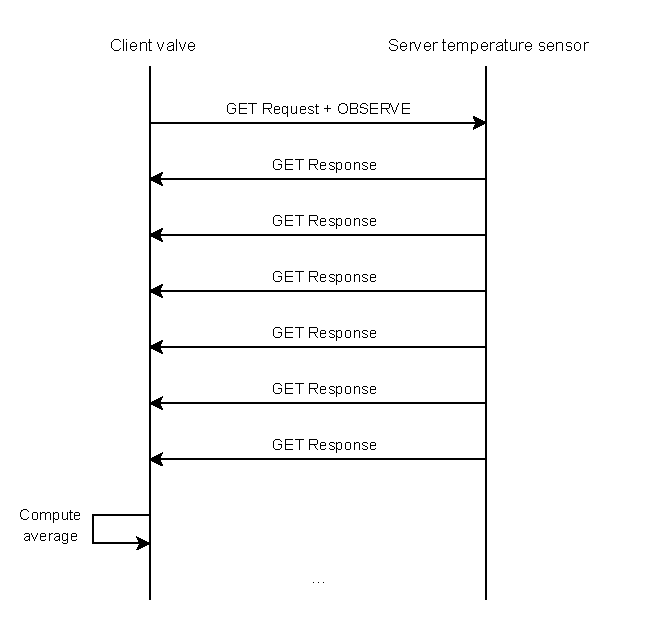
\includegraphics[width=\linewidth, height=0.5\textheight, keepaspectratio]{coap.pdf}
    \caption{Message flow CoAP}
\end{figure}
We start the energy consumption calculation by computing the number of sensor readings, $N_{sensor\_read}$, and the number of computations of the average, $N_{avg}$.
\[N_{sensor\_read} = (24\text{ h}  \cdot 60 \text{ min/h}) / 5 \text{ min} = 288\]
\[N_{avg} = (24\text{ h}  \cdot 60 \text{ min/h}) / 30 \text{ min} = 48\]

We can compute the energy consumed by the two devices as:
\[E_{CoAP\_valve} = E_{TX} \cdot L_{GET\_Req} + N_{sensor\_read} \cdot E_{RX} \cdot L_{GET\_Resp} + N_{avg} \cdot E_{C} = 122.574 \text{ mJ}\]
\[E_{CoAP\_sensor} = E_{RX} \cdot L_{GET\_Req} + N_{sensor\_read} \cdot E_{TX} \cdot L_{GET\_Resp} = 6.364 \text{ mJ}\]
\[E_{CoAP\_total} = E_{CoAP\_valve} + E_{CoAP\_sensor} = 128.938 \text{ mJ}\]

\section{EQ1.b Energy consumed using MQTT}
In this section, we compute the energy consumption if the devices communicate through MQTT. In this scenario, the Raspberry Pi acts as MQTT Broker, the sensor is a Publisher and the valve is a Subscriber. In order to minimize energy consumption, we adopt the following configurations:
\begin{itemize}
\item Messages are exchanged with QoS 0, in "at most once" mode, i.e. no PUBACK messages are exchanged.
\item Neither the sensor nor the valve send ping messages. The sensor uses a Keep Alive greater than 5 minutes, so that the periodic PUBLISH message will reset the timer. The valve, instead, uses a Keep Alive 0, which disables the Keep Alive mechanism; disconnections from the valve will be detected at TCP level when the broker will try to communicate the new sensor reading but won't be able to reach the valve.
\end{itemize}
The sensor (Publisher) connects to the Broker and starts publishing temperature values every 5 minutes. The valve (Subscriber) connects to the Broker, subscribes to the topic and starts receiving temperature values.
\begin{figure}[H]
    \centering
    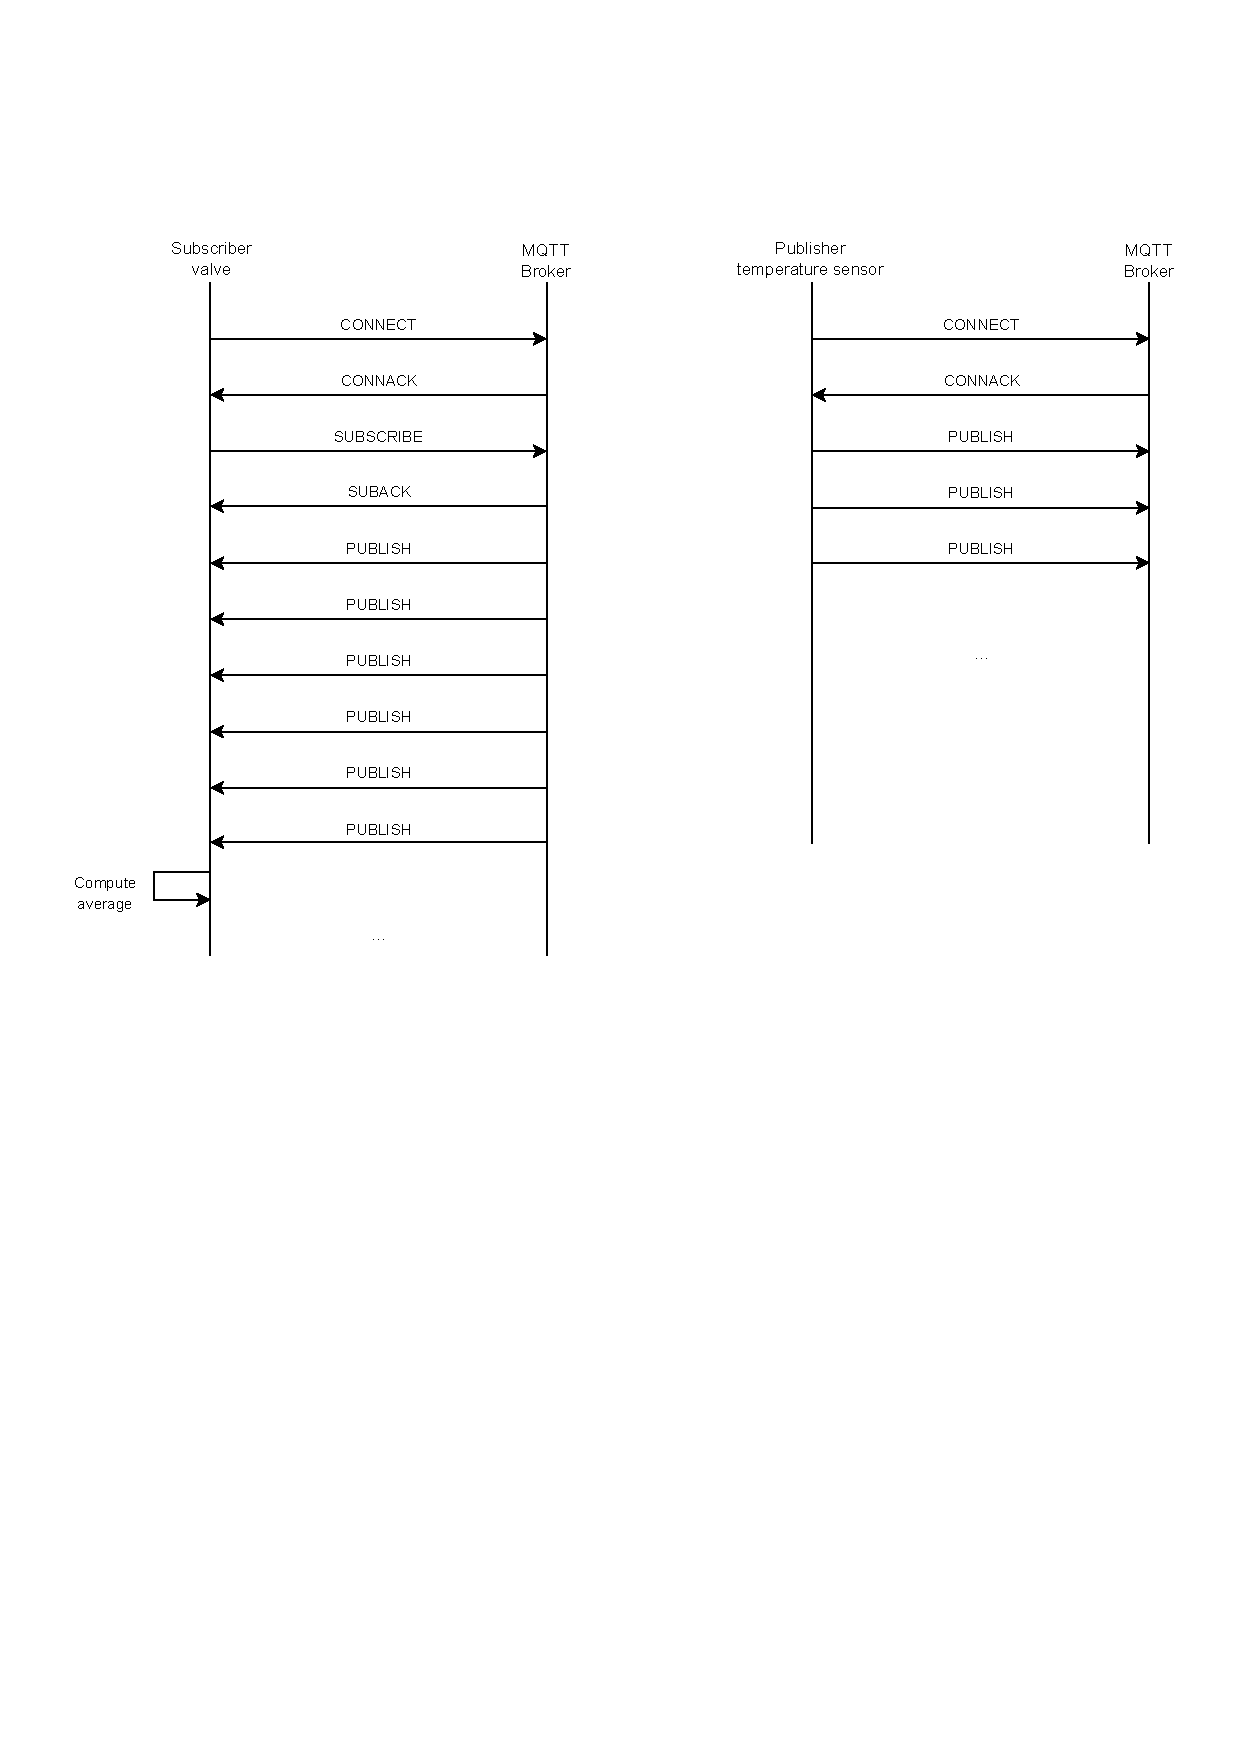
\includegraphics[width=\linewidth, height=0.5\textheight, keepaspectratio]{mqtt.pdf}
    \caption{Message flow MQTT}
\end{figure}
We can compute the energy consumed by the two devices as:
\[E_{MQTT\_valve} = E_{TX} \cdot L_{CONNECT} + E_{RX} \cdot L_{CONNACK} + E_{TX} \cdot L_{SUBSCRIBE} +\]
\[+ E_{RX} \cdot L_{SUBACK} + N_{sensor\_read} \cdot E_{RX} \cdot L_{PUBLISH} + N_{avg} \cdot E_{C} = 124.378 \text{ mJ}\]
\[E_{MQTT\_sensor} = E_{TX} \cdot L_{CONNECT} + E_{RX} \cdot L_{CONNACK} + N_{sensor\_read} \cdot E_{TX} \cdot L_{PUBLISH} =\]
\[= 7.877 \text{ mJ}\]
\[E_{MQTT\_total} = E_{MQTT\_valve} + E_{MQTT\_sensor} = 132.255 \text{ mJ}\]

\section{EQ2 Improvements}
In this section, we propose two ways to decrease the energy consumed by the two device while using the Raspberry Pi as a broker. 

\subsection{Using MQTT-SN}
The first improvement consists in using MQTT-SN instead of MQTT. Since we have not been provided with exact values for MQTT-SN messages we are going to make some assumptions. We assume that the size of the PUBLISH message is:
\[L_{PUBLISH\_MQTT\_SN} = L_{PUBLISH\_MQTT} - L_{TOPIC\_MQTT} + L_{TOPIC\_MQTT\_SN}  =\]
\[= 68 \text{ B} - 10 \text{ B} + 2 \text{ B} = 60 \text{ B} \]
Moreover we assume that the size of REGISTER is 59 B and the size of REGISTER ACK is 51 B, as seen during the exercise session.\\
Using MQTT-SN introduces a trade-off: 
\begin{itemize}
	\item Disadvantage: the Publisher needs to send a REGISTER message to the broker, represented by the Raspberry Pi, before being able to send PUBLISH messages.
	\item Advantage: PUBLISH messages have a reduced size, since they have a 2 Bytes long topic, instead of the 10 Bytes long one of MQTT messages.
\end{itemize}
On the long run, using MQTT-SN is beneficial, since we send more messages and compensate the initial cost of the REGISTER message with the lowered cost of PUBLISH messages. We start by computing the number of packets that the Publisher should send with MQTT-SN in order to save energy with respect to MQTT. To do so, we compute the energy needed to send the initial packages, publish a variable number of packages m and compute the average every 30 minutes both with MQTT and MQTT-SN.\\
\begin{figure}[H]
    \centering
    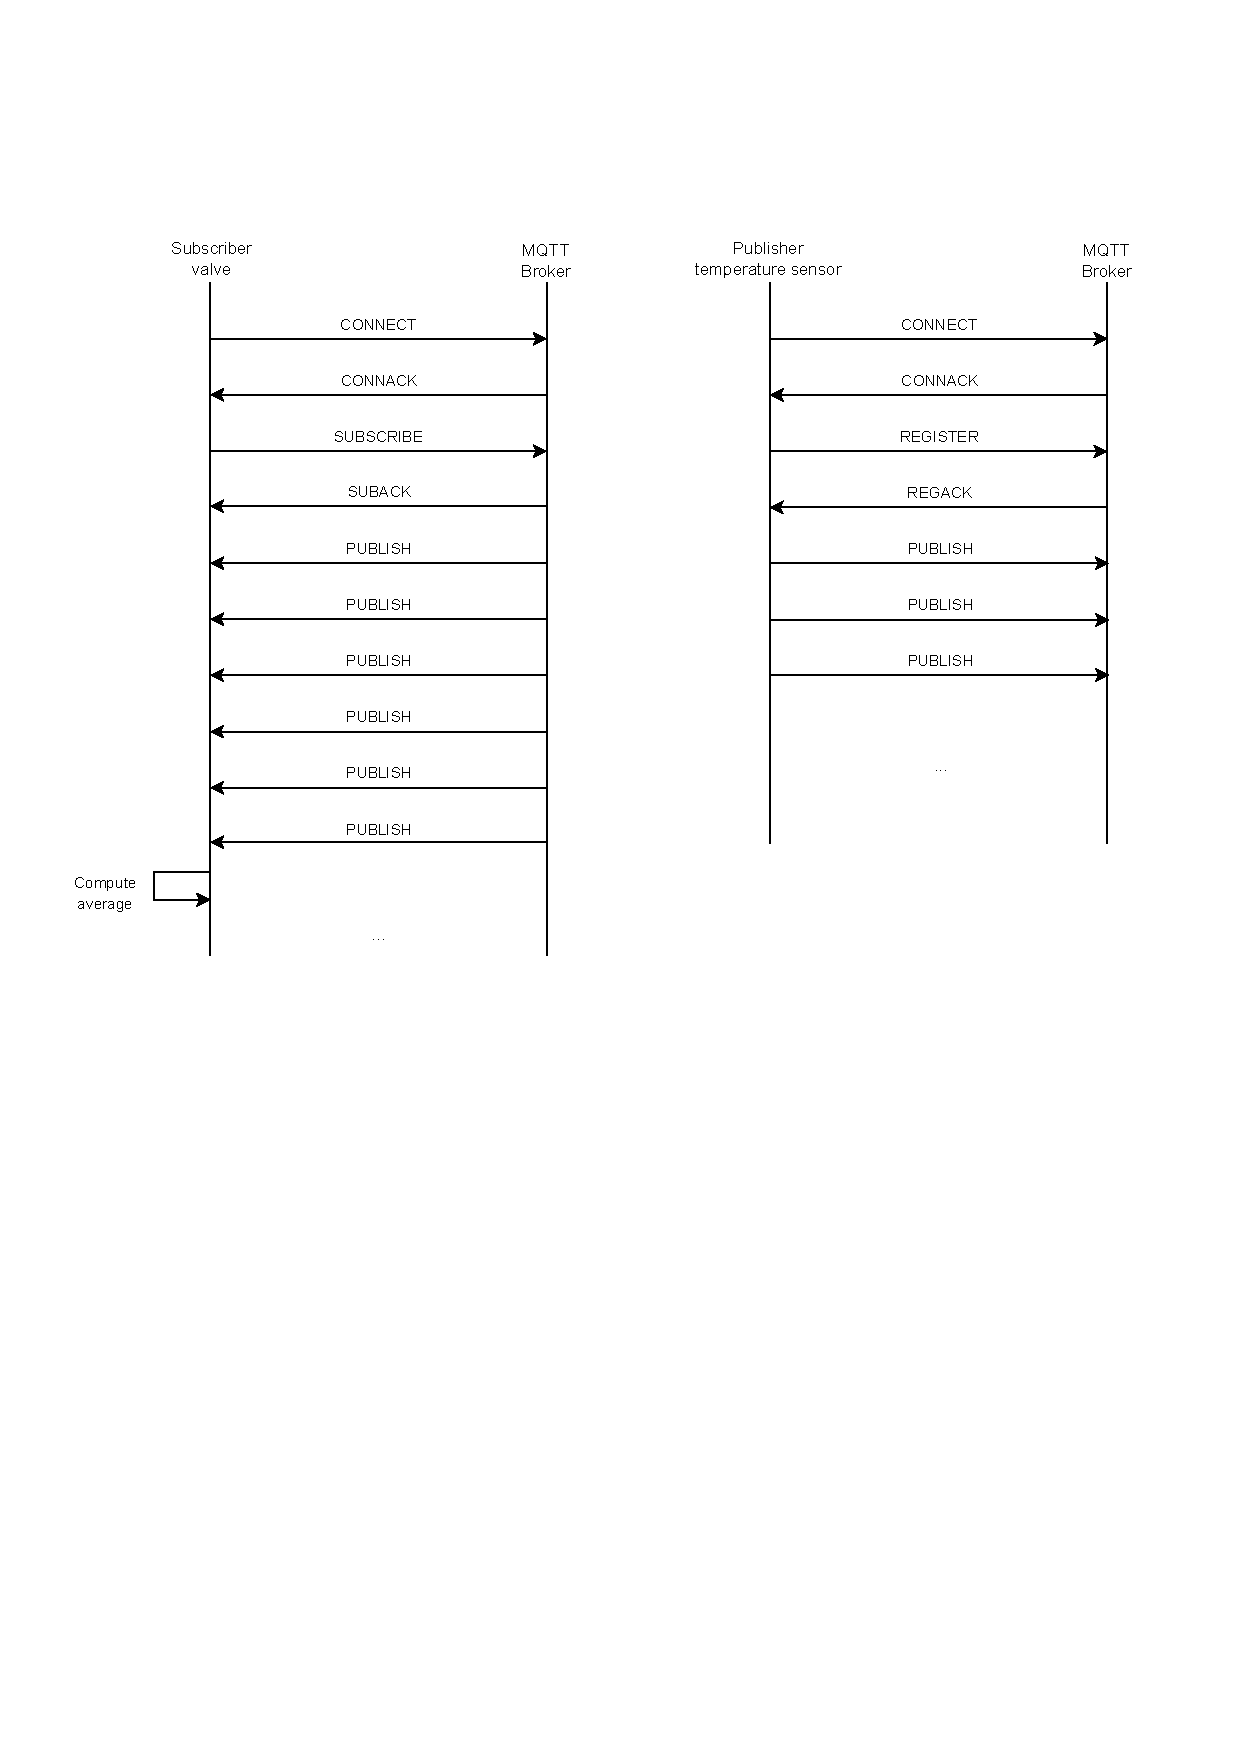
\includegraphics[width=\linewidth, height=0.5\textheight, keepaspectratio]{mqtt_sn.pdf}
    \caption{Message flow MQTT-SN}
\end{figure}
The energy consumption to send m packets with MQTT is:
\[E_{MQTT\_valve} = E_{TX} \cdot L_{CONNECT} + E_{RX} \cdot L_{CONNACK} + E_{TX} \cdot L_{SUBSCRIBE} +\]
\[+ E_{RX} \cdot L_{SUBACK} + m \cdot E_{RX} \cdot L_{PUBLISH} + N_{avg} \cdot E_{C} = 115.291 \text{ mJ} + m \cdot 3.1552 \cdot 10^{-5} \text{ J}\]
\[E_{MQTT\_sensor} = E_{TX} \cdot L_{CONNECT} + E_{RX} \cdot L_{CONNACK} + m \cdot E_{TX} \cdot L_{PUBLISH} =\]
\[= 4.3408 \cdot 10^{-5} \text{ J} + m \cdot 2.72 \cdot 10^{-5} \text{ J}\]

The energy consumption to send m packets in MQTT-SN is:
\[E_{MQTT\_SN\_valve} = E_{TX} \cdot L_{CONNECT} + E_{RX} \cdot L_{CONNACK} + E_{TX} \cdot L_{SUBSCRIBE} +\]
\[+ E_{RX} \cdot L_{SUBACK} + m \cdot E_{RX} \cdot L_{PUBLISH} + N_{avg} \cdot E_{C} = 115.291 \text{ mJ} + m \cdot 2.784 \cdot 10^{-5} \text{ J}\]
\[E_{MQTT\_SN\_sensor} = E_{TX} \cdot L_{CONNECT} + E_{RX} \cdot L_{CONNACK} + E_{TX} \cdot L_{REGISTER} +\]
\[+ E_{RX} \cdot L_{REGACK} + m \cdot E_{TX} \cdot L_{PUBLISH} = 9.0672 \cdot 10^{-5} \text{ J} + m \cdot 2.4 \cdot 10^{-5} \text{ J}\]

We now find the number of packets that the publisher should publish in order for the communication to be cheaper with MQTT-SN.\\
For the valve:
\[E_{MQTT\_SN\_valve} \leq E_{MQTT\_valve} \]
\[115.291 \text{ mJ} + m \cdot 2.784 \cdot 10^{-5} \text{ J}  \leq 115.291 \text{ mJ} + m \cdot 3.1552 \cdot 10^{-5} \text{ J}\]
Which is true for every value of m, i.e. the valve always consumes less energy using MQTT-SN over MQTT.\\
For the sensor, instead:
\[E_{MQTT\_SN\_sensor} \leq E_{MQTT\_sensor}\]
\[9.0672 \cdot 10^{-5} \text{ J} + m \cdot 2.4 \cdot 10^{-5} \text{ J} \leq 4.3408 \cdot 10^{-5} \text{ J} + m \cdot 2.72 \cdot 10^{-5} \text{ J}\]
Which is true for $m \geq 14.77$, i.e. MQTT-SN is convenient if the publisher sends 15 packets or more.

Since the sensor sends 288 PUBLISH messages, using MQTT-SN is convenient. The energy consumption using MQTT-SN is computed by substituting $m = 288$:
\[E_{MQTT\_SN\_valve} = 123.309 \text{ mJ}\]
\[E_{MQTT\_SN\_sensor} = 7.003 \text{ mJ}\]
\[E_{MQTT\_SN\_total} = 130.093 \text{ mJ}\]
We can see that the new energy consumption is smaller than the one computed using MQTT, as expected by our calculations on the minimum number of packets m.

\subsection{Sending less frequent updates}
Another strategy we can adopt to reduce the energy consumption is to reduce the rate with which the sensor sends updates to the valve. The valve still computes the average every 30 minutes, but with 3 new readings, instead of 5, so the result will be less precise. The trade-off in this case is between saving energy and having an accurate measurement of the average.\\
For example, the sensor can send a temperature reading to the valve every 10 minutes. In this case, the number of readings published by the sensor will be:
\[N_{sensor\_read} = (24\text{ h}  \cdot 60 \text{ min/h}) / 10 \text{ min} = 144\]
Since 144 is stil greater than 15, using MQTT-SN is better than MQTT, so we can compute the new energy consumption by using $m = 144$:
\[E_{MQTT\_SN\_valve} = 119.300 \text{ mJ}\]
\[E_{MQTT\_SN\_sensor} = 3.547 \text{ mJ}\]
\[E_{MQTT\_SN\_total} = 122.847 \text{ mJ}\]


